\chapter{Mise en Oeuvre}
\label{chap:mise-en-oeuvre}

\section{Configuration initiale des FortiGate}

\subsection{Interfaces réseau}

J'ai commencé par configurer les interfaces réseau en ligne de commande (CLI) via Telnet \cite{1}. Chaque FortiGate utilise ses 3 ports disponibles : port1 (WAN), port2 (LAN), port3 (HA Heartbeat).

\begin{lstlisting}[language=bash, caption={Configuration des interfaces FGT-Primary}]
config system interface
    edit "port1"
        set mode dhcp
        set allowaccess ping https ssh
    next
    edit "port2"
        set ip 192.168.10.1 255.255.255.0
        set allowaccess ping https ssh
    next
    edit "port3"
        set ip 169.254.0.1 255.255.255.252
        set allowaccess ping
    next
end
\end{lstlisting}

\begin{lstlisting}[language=bash, caption={Configuration des interfaces FGT-Secondary}]
config system interface
    edit "port1"
        set mode dhcp
        set allowaccess ping https ssh
    next
    edit "port2"
        set ip 192.168.20.1 255.255.255.0
        set allowaccess ping https ssh
    next
    edit "port3"
        set ip 169.254.0.2 255.255.255.252
        set allowaccess ping
    next
end
\end{lstlisting}

\noindent\textit{Choix technique :} La licence d'évaluation limite l'appareil à 3 interfaces. J'ai alloué port1 (DHCP) pour le WAN, port2 pour le LAN client, et port3 pour le heartbeat HA. Cette contrainte a dicté l'ensemble de la topologie.

\begin{figure}[H]
\centering
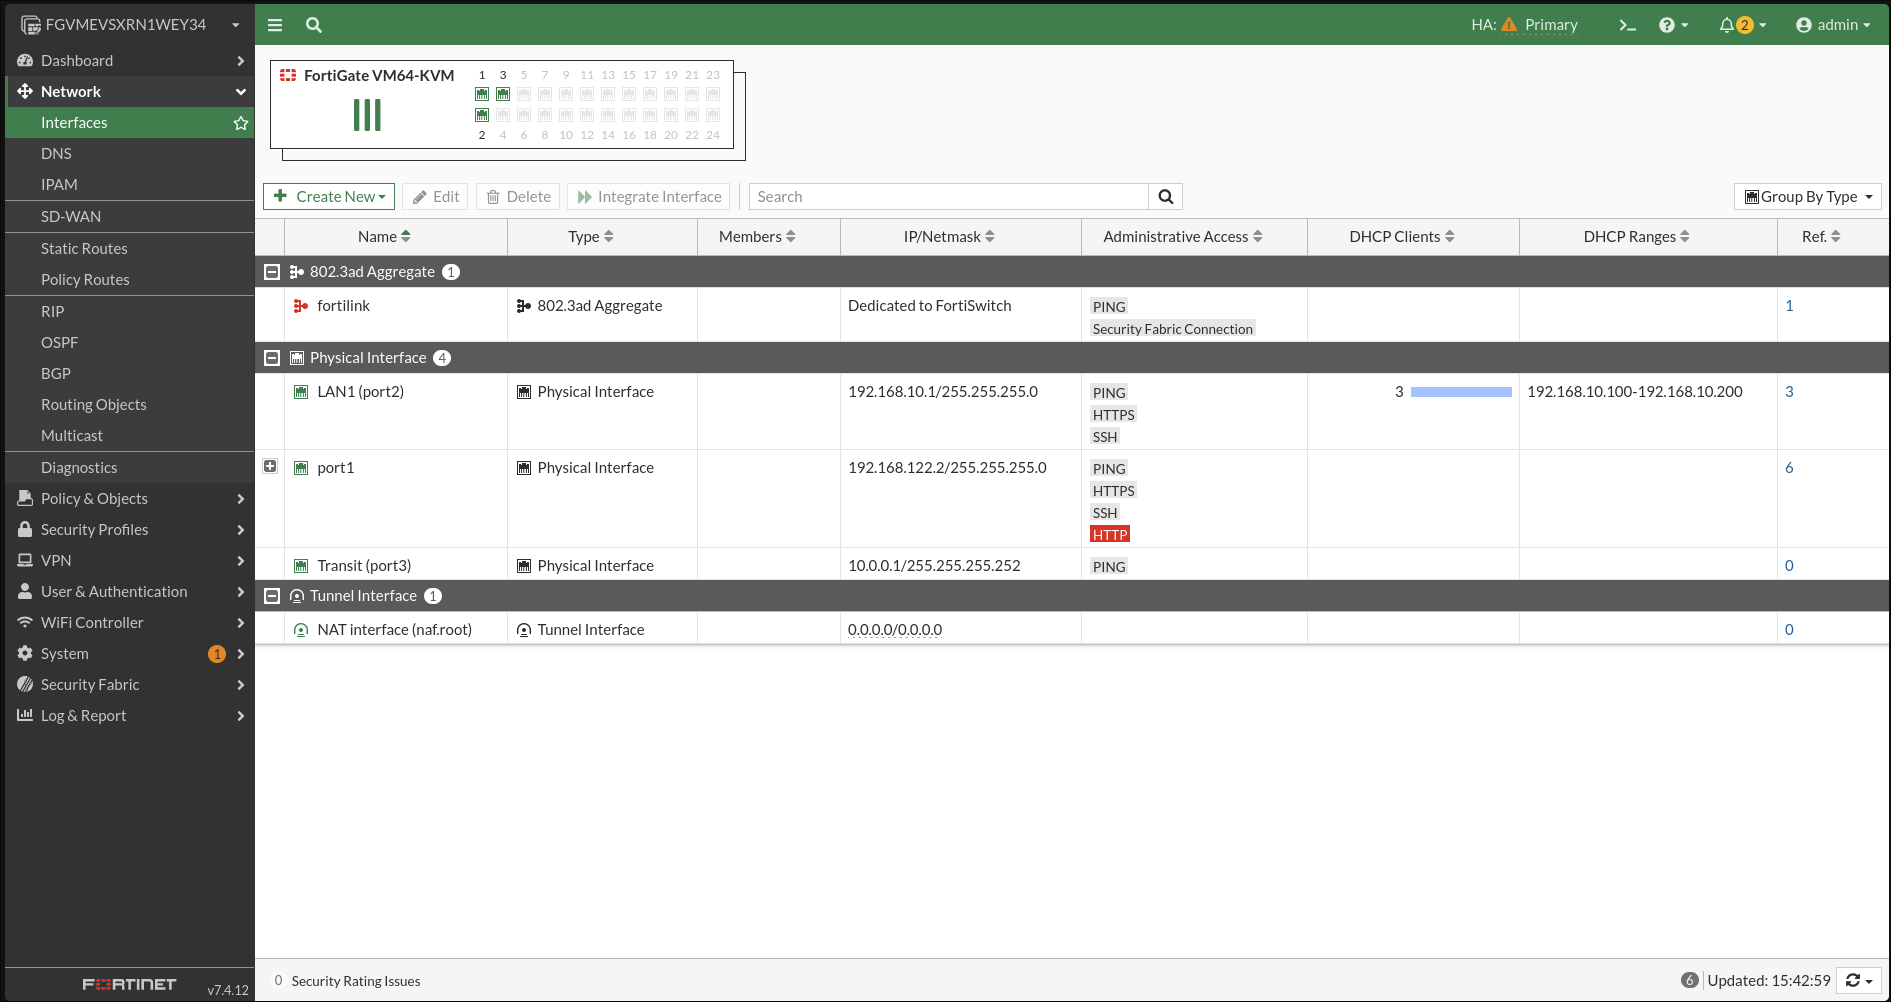
\includegraphics[width=0.9\textwidth]{images/interfaces-fgtp.png}
\caption{Configuration des interfaces --- FGT-Primary}
\label{fig:interfaces-fgtp}
\end{figure}

\subsection{DHCP sur les LANs}

Chaque FortiGate gère le DHCP pour son segment LAN :

\begin{lstlisting}[language=bash, caption={Serveur DHCP FGT-Primary pour LAN1}]
config system dhcp server
    edit 1
        set interface "port2"
        set default-gateway 192.168.10.1
        set netmask 255.255.255.0
        config ip-range
            edit 1
                set start-ip 192.168.10.100
                set end-ip 192.168.10.200
            next
        end
        set dns-service default
    next
end
\end{lstlisting}

\subsection{Route par défaut}

\begin{lstlisting}[language=bash, caption={Route par défaut vers Internet}]
config router static
    edit 1
        set device "port1"
        set gateway 192.168.122.1
    next
end
\end{lstlisting}

\section{Firewall policies}

La politique principale permet le trafic LAN vers Internet avec masquage (SNAT) :

\begin{lstlisting}[language=bash, caption={Politique LAN1 vers WAN}]
config firewall policy
    edit 1
        set name "LAN1-to-WAN"
        set srcintf "port2"
        set dstintf "port1"
        set srcaddr "all"
        set dstaddr "all"
        set action accept
        set schedule "always"
        set service "HTTP" "HTTPS" "DNS" "PING"
        set logtraffic all
        set nat enable
    next
end
\end{lstlisting}

\begin{lstlisting}[language=bash, caption={Politique LAN2 vers WAN}]
config firewall policy
    edit 2
        set name "LAN2-to-WAN"
        set srcintf "port2"
        set dstintf "port1"
        set srcaddr "all"
        set dstaddr "all"
        set action accept
        set schedule "always"
        set service "HTTP" "HTTPS" "DNS" "PING"
        set logtraffic all
        set nat enable
    next
end
\end{lstlisting}

\noindent\textit{Analyse :} Avec seulement 3 politiques disponibles, j'ai dû prioriser : (1) LAN vers WAN pour l'accès Internet, (2) LAN vers LAN via le Docker Router pour le routage inter-LAN, (3) une politique de gestion. Cette contrainte m'a forcé à concevoir un réseau minimaliste mais fonctionnel.

\begin{figure}[H]
\centering
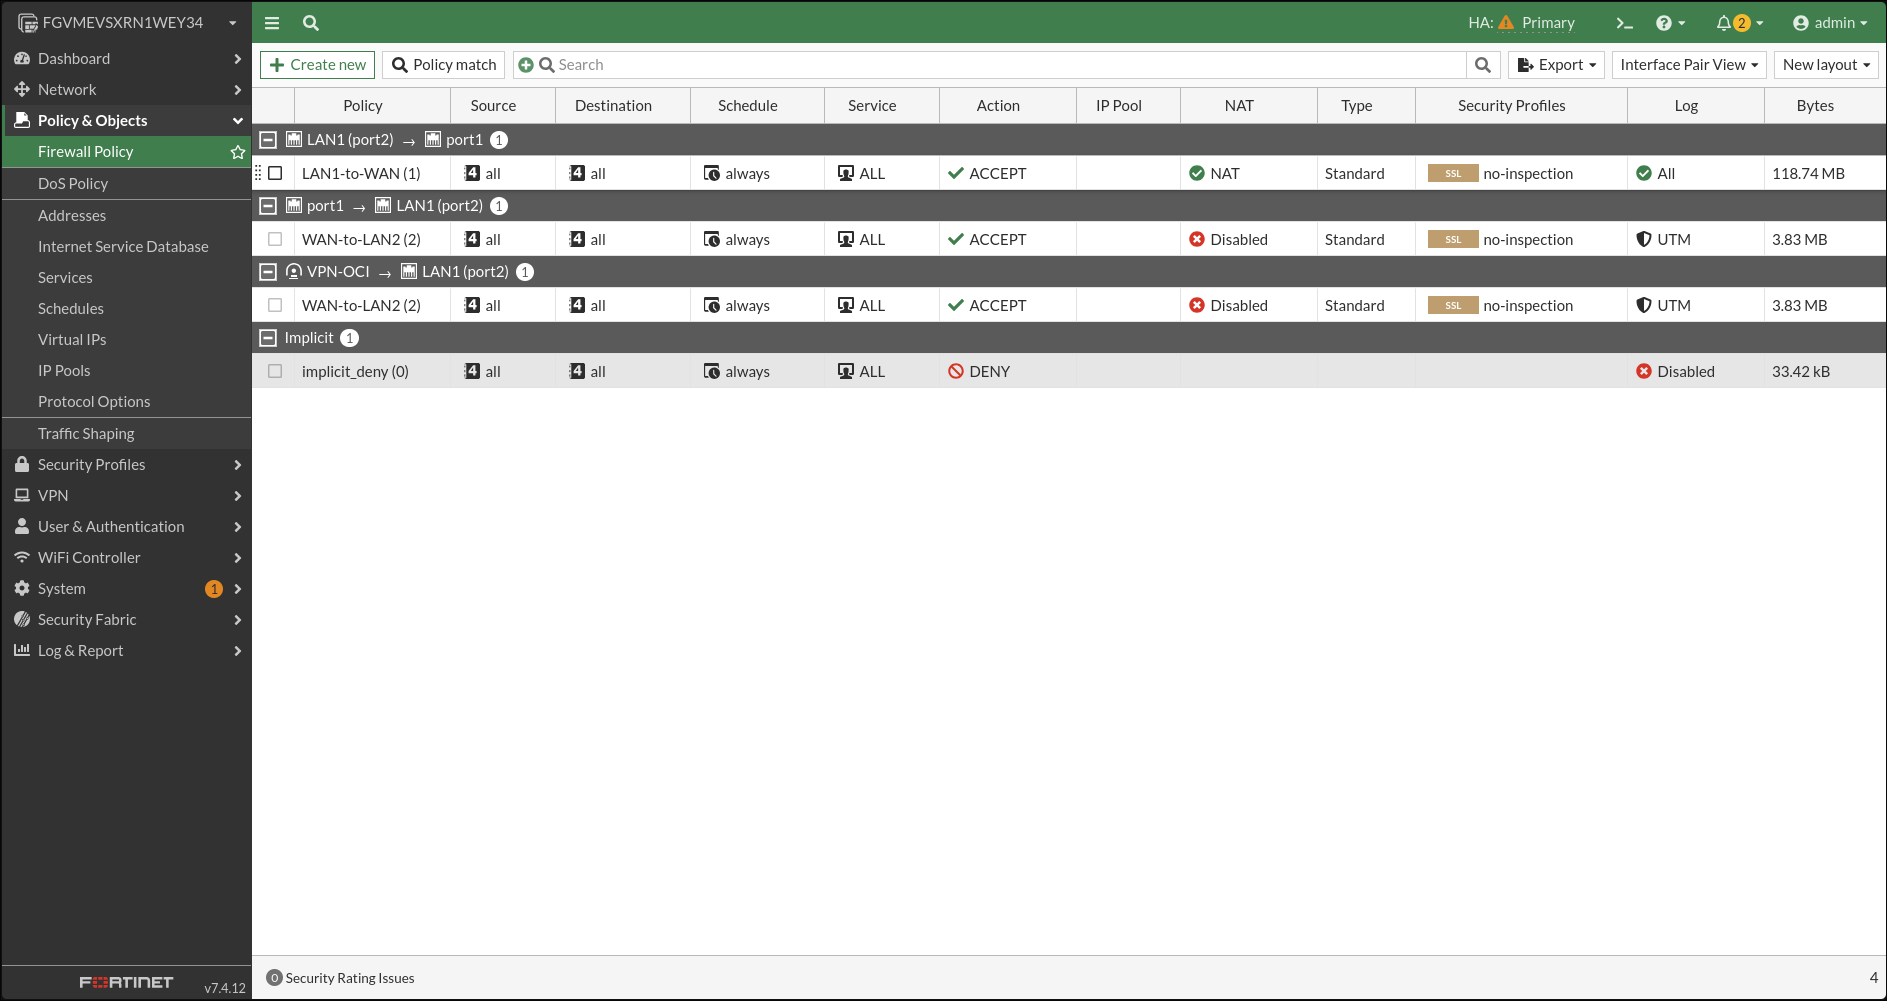
\includegraphics[width=0.9\textwidth]{images/politiques-fw.png}
\caption{Politiques firewall --- Vue d'ensemble}
\label{fig:politiques-fw}
\end{figure}

\section{High Availability}

\subsection{Configuration HA Active-Passive}

\begin{lstlisting}[language=bash, caption={Configuration HA --- FGT-Primary (actif)}]
config system ha
    set group-name "FortiLab-HA"
    set mode a-p
    set hbdev "port3"
    set priority 200
    set session-sync-dev "port3"
end
\end{lstlisting}

\begin{lstlisting}[language=bash, caption={Configuration HA --- FGT-Primary-HA (passif)}]
config system ha
    set group-name "FortiLab-HA"
    set mode a-p
    set hbdev "port3"
    set priority 100
    set session-sync-dev "port3"
end
\end{lstlisting}

\noindent\textit{Justification du mode Active-Passive :} J'ai choisi le mode actif-passif plutôt qu'actif-actif pour trois raisons : (1) le mode actif-actif nécessite des interfaces supplémentaires pour la répartition de charge, incompatible avec la limite de 3 ports ; (2) le mode actif-passif est plus simple à déboguer ; (3) pour un environnement de taille réduite, la redondance suffit sans parallélisme du trafic.

La même configuration est appliquée au second cluster (FGT-Secondary + FGT-Secondary-HA).

\begin{figure}[H]
\centering
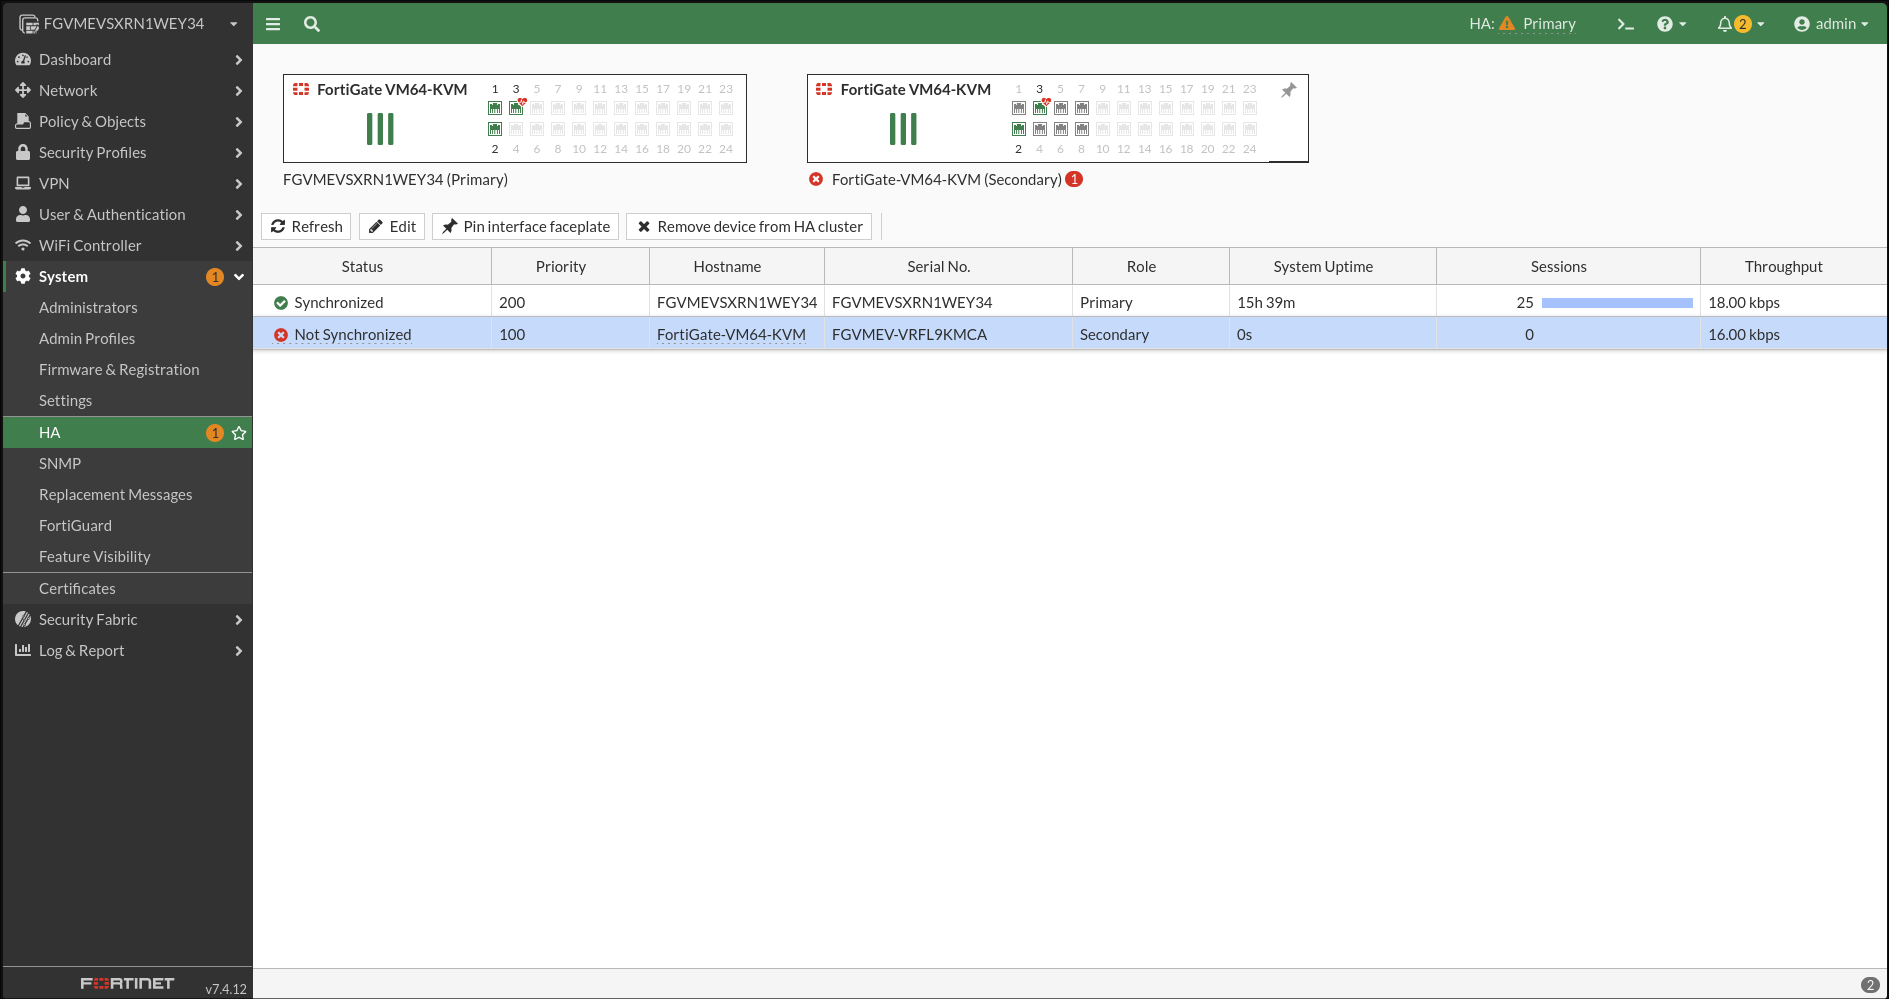
\includegraphics[width=0.9\textwidth]{images/ha-status.png}
\caption{Statut du cluster HA --- FGT-Primary actif}
\label{fig:ha-status}
\end{figure}

\section{Docker Router --- Routage cross-LAN}

Le Docker Router remplace le lien transit OSPF et assure le routage entre LAN1 et LAN2 :

\begin{lstlisting}[language=bash, caption={Configuration du Docker Router}]
# Interfaces
ip addr add 192.168.10.254/24 dev eth0
ip addr add 192.168.20.254/24 dev eth1
ip link set eth0 up
ip link set eth1 up

# Activation du forwarding
echo 1 > /proc/sys/net/ipv4/ip_forward

# Routage statique (ou OSPF/BGP via FRR)
ip route add 192.168.10.0/24 dev eth0
ip route add 192.168.20.0/24 dev eth1
\end{lstlisting}

\noindent\textit{Analyse :} Le Docker Router a été préféré au transit OSPF direct entre les FortiGate pour plusieurs raisons : (1) il libère le port3 pour le heartbeat HA ; (2) il permet de démontrer le routage inter-LAN avec un équipement séparé ; (3) il est léger (quelques Mo de RAM) et rapide à déployer.

\begin{figure}[H]
\centering
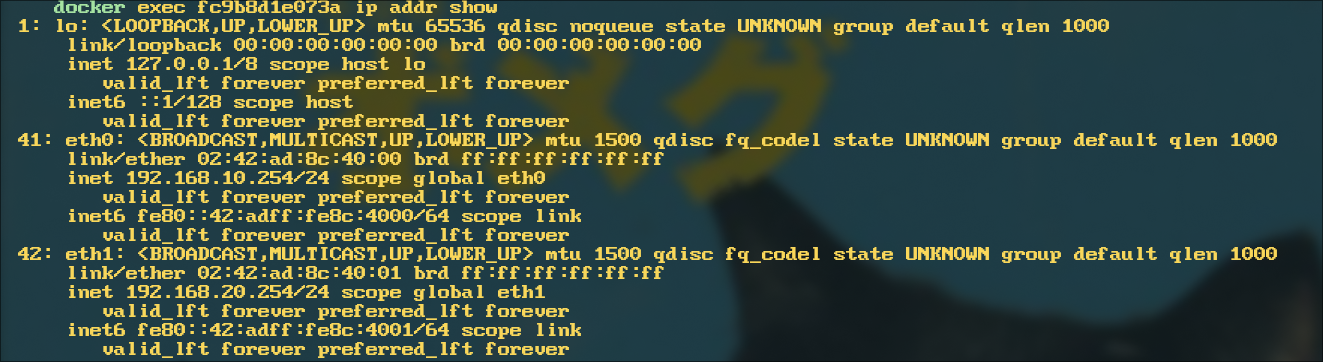
\includegraphics[width=0.9\textwidth]{images/docker-router.png}
\caption{Docker Router --- Routage cross-LAN}
\label{fig:docker-router}
\end{figure}

\section{NAT (Network Address Translation)}

J'ai configuré le NAT sortant (SNAT) via la politique firewall avec l'option \texttt{set nat enable}. Cela masque l'adresse source des clients LAN derrière l'adresse du port WAN du FortiGate.

\section{VPN --- Contraintes et limitations}

\subsection{IPSec VPN}

L'objectif initial était d'établir un tunnel IPSec site-à-site avec un endpoint cloud. Cette fonctionnalité n'a pas pu être finalisée pour deux raisons :

\begin{enumerate}
    \item \textbf{Licence d'évaluation :} FortiOS en mode eval impose des chiffrements faibles (DES/SHA1) et limite le nombre de configurations réseau. Les commandes standard de négociation IKEv2 (\texttt{set proposal aes256-sha256}, \texttt{execute vpn tunnel up}) échouent avec des erreurs de syntaxe.
    \item \textbf{Firewall cloud :} Les paquets IKE\_SA\_INIT sont interceptés par le firewall virtuel du provider cloud avant d'atteindre l'endpoint, en raison de restrictions au niveau du réseau virtuel.
\end{enumerate}

\noindent\textit{Leçon apprise :} Cette expérience m'a permis de comprendre les défis de l'interconnexion entre un environnement local et le cloud, y compris les contraintes de licence, les problèmes de NAT traversal et la configuration des firewalls cloud.

\subsection{VPN SSL}

Le VPN SSL n'a pas été implémenté en raison de la limite de 3 interfaces de la licence eval. L'interface virtuelle ssl.root nécessite une configuration préalable du certificat serveur et des pools d'adresses, ce qui dépasse les ressources disponibles de l'environnement de test.

\section{Profils de sécurité}

\subsection{Profils de sécurité --- Limites de la licence eval}

Les profils de sécurité (antivirus, IPS, Web Filter, DNS Filter, SSL Inspection) sont disponibles sur FortiGate même en mode évaluation. Cependant, trois contraintes majeures limitent leur utilisation :

\begin{enumerate}
    \item \textbf{Signatures factory} : sans licence FortiGuard, les moteurs AV et IPS utilisent uniquement les signatures pré-installées (factory). Ces signatures couvrent les menaces les plus courantes mais ne sont pas mises à jour.
    \item \textbf{Limite de 3 politiques firewall} : les profils UTM doivent être attachés à des politiques. Avec seulement 3 politiques disponibles (LAN1→WAN, LAN2→WAN, cross-LAN), il n'y a pas de marge pour tester différents combos de profils.
    \item \textbf{SSL Inspection} : un certificat CA auto-signé a été généré, mais l'inspection SSL n'a pas été appliquée aux politiques en raison de la même contrainte de 3 politiques.
\end{enumerate}

\noindent\textit{Leçon apprise :} Cette expérience m'a permis de comprendre l'importance d'une licence FortiGuard pour un pare-feu FortiGate en production. Sans elle, les profils de sécurité sont réduits à leur minimum et ne peuvent pas démontrer leur pleine valeur.

\subsection{Antivirus --- Test EICAR}

Le fichier EICAR (European Institute for Computer Antivirus Research) est un fichier test standard reconnu par tous les moteurs antivirus. L'endpoint \texttt{/eicar} existe sur l'application Docker Flask, mais le moteur AV du FortiGate ne dispose pas de mises à jour de signatures FortiGuard pour détecter les menaces en temps réel.

\subsection{IPS --- Signatures factory}

Les signatures IPS factory couvrent les attaques les plus courantes (SQL Injection, XSS, scan de ports). Cependant, sans mise à jour FortiGuard, les signatures ne couvrent pas les variantes récentes des attaques.

\subsection{Web Filter et DNS Filter --- Configurations statiques}

Sans FortiGuard, le filtrage URL et DNS repose exclusivement sur des listes statiques définies manuellement. La catégorisation automatique des sites (phishing, malware, etc.) n'est pas disponible.

\subsection{SSL Inspection --- Certificat CA généré}

Un certificat CA auto-signé a été généré localement pour déchiffrer le trafic HTTPS. Cependant, l'inspection SSL n'a pas été appliquée aux politiques firewall en raison de la limite de 3 politiques imposée par la licence eval.

\section{Services Docker}

\subsection{PostgreSQL}

J'ai configuré la base de données PostgreSQL avec :
\begin{itemize}
    \item \textbf{Image} : postgres:16-alpine
    \item \textbf{IP} : 192.168.10.11/24 (statique)
    \item \textbf{Base} : labdb
    \item \textbf{Utilisateur} : labuser / gns3lab
    \item \textbf{Tables} : users (14 lignes), requests
\end{itemize}

\subsection{appServer}

Le serveur d'application Flask expose les endpoints suivants :
\begin{itemize}
    \item \texttt{GET /} : page d'accueil
    \item \texttt{GET /health} : vérification de santé
    \item \texttt{GET /db-check} : test de connexion à la base
    \item \texttt{GET /inspect} : démonstration NAT
    \item \texttt{GET /eicar} : test antivirus
    \item \texttt{GET /attack?sql=payload} : test IPS (SQLi)
    \item \texttt{GET /attack?xss=payload} : test IPS (XSS)
\end{itemize}

\noindent\textit{Pourquoi Docker plutôt que des VMs :} J'ai utilisé Docker pour les services applicatifs (PostgreSQL, Flask) au lieu de machines virtuelles séparées car : (1) les conteneurs démarrent en quelques secondes contre plusieurs minutes pour des VMs ; (2) l'empreinte mémoire est réduite ($\approx$50 MB par conteneur vs $\approx$1 GB par VM) ; (3) Docker s'intègre nativement avec GNS3 via le connecteur bridge ; (4) les images sont reproductibles et partageables.

\subsection{Grafana et Prometheus}

Le stack de supervision comprend :
\begin{itemize}
    \item \textbf{Prometheus} : collecte de métriques (192.168.20.12:9090)
    \item \textbf{Grafana} : tableaux de bord (192.168.20.11:3000)
    \item Intégration des métriques réseau et système
\end{itemize}

\begin{figure}[H]
\centering
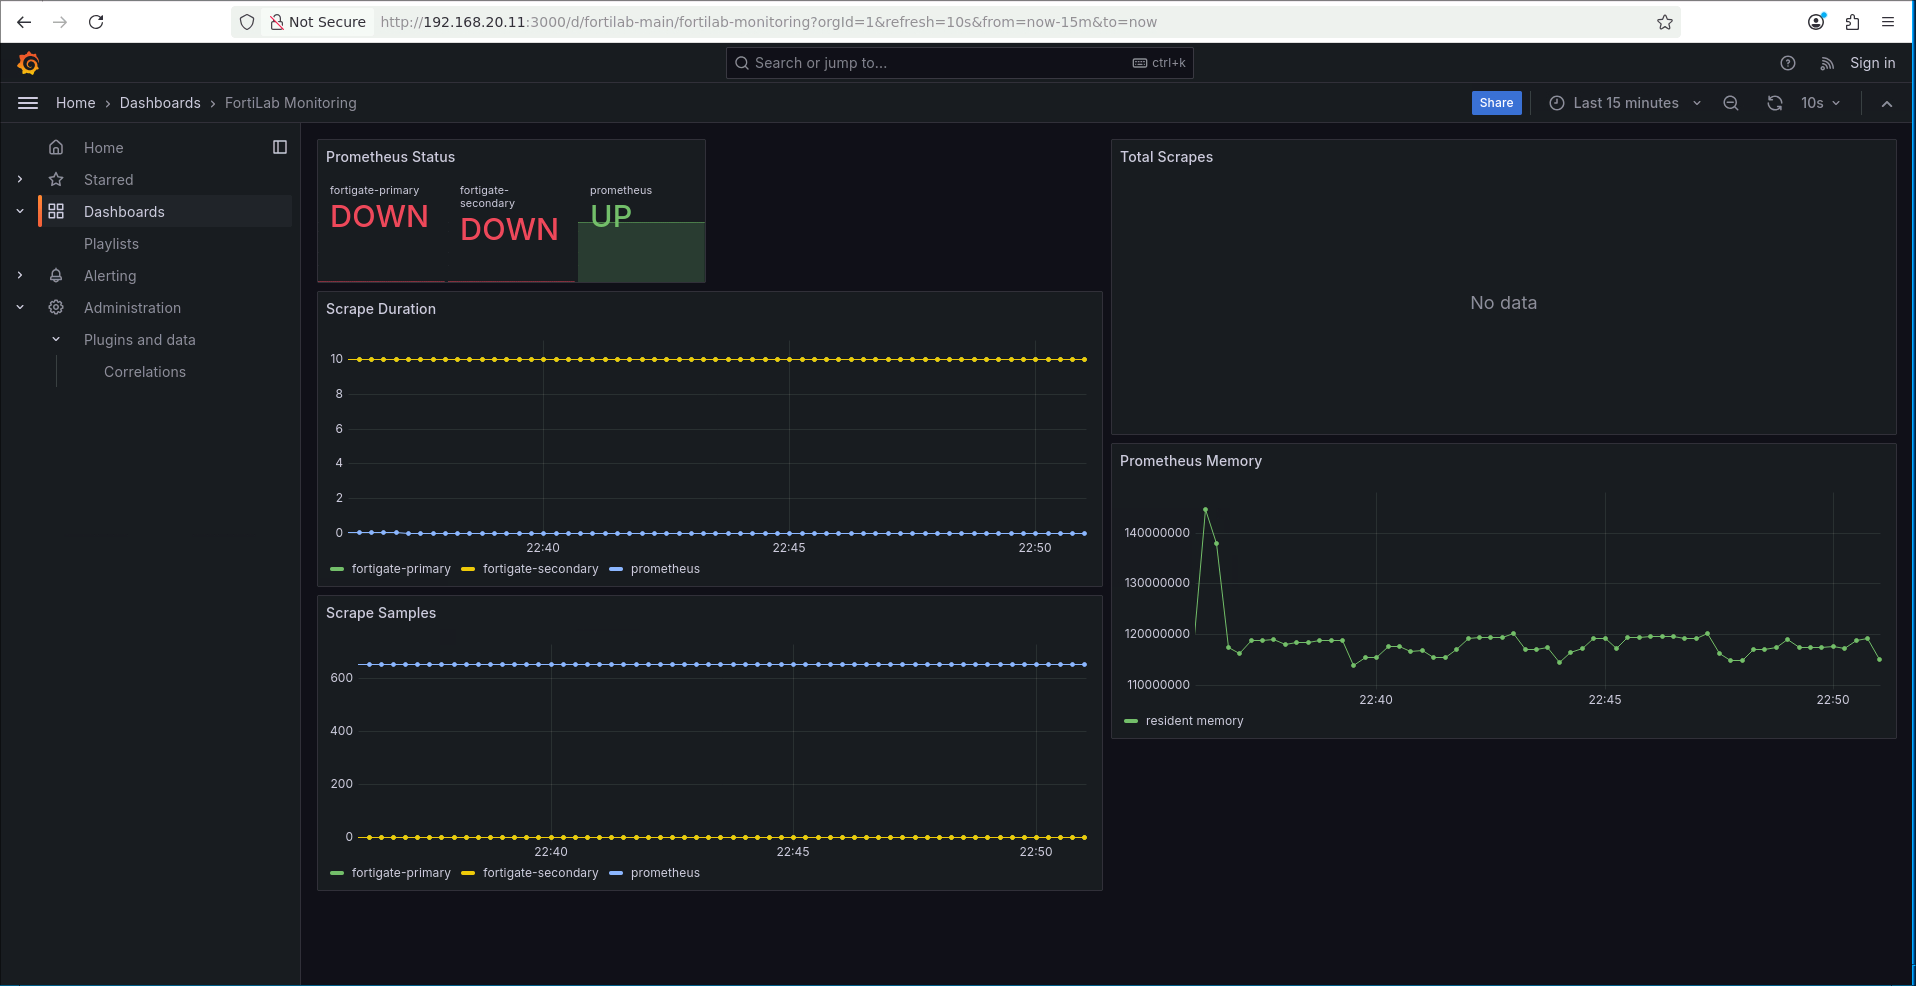
\includegraphics[width=0.9\textwidth]{images/grafana-dashboard.png}
\caption{Grafana --- Tableau de bord de supervision}
\label{fig:grafana-dashboard}
\end{figure}

\section{Journalisation et monitoring}

Le logging centralisé est assuré par syslog (BSD, UDP 514) et Grafana pour les tableaux de bord.
